\documentclass[12pt]{report}  

\usepackage[utf8]{inputenc}
\usepackage{amsmath, amssymb}
\usepackage{graphicx}
\usepackage{hyperref}
\usepackage{geometry}
\geometry{margin=1in}
\usepackage{caption}
\usepackage{float}
\usepackage{enumitem}
\usepackage{tocloft}
\usepackage{tcolorbox}  
\usepackage{amssymb}
\usepackage{listings}
\usepackage{xcolor}
\usepackage[T1]{fontenc}
\usepackage{lmodern}

\usepackage{booktabs}  % cho \toprule, \midrule, \bottomrule
\usepackage{tabularx}  % cho cột X tự động giãn
          

\definecolor{codegreen}{rgb}{0,0.6,0}
\definecolor{codegray}{rgb}{0.5,0.5,0.5}
\definecolor{codepurple}{rgb}{0.58,0,0.82}
\definecolor{backcolour}{rgb}{0.95,0.95,0.92}
\usepackage{hyperref}
\hypersetup{plainpages=false}

\lstdefinestyle{mystyle}{
	backgroundcolor=\color{backcolour},   
	commentstyle=\color{codegreen},
	keywordstyle=\color{magenta},
	numberstyle=\tiny\color{codegray},
	stringstyle=\color{codepurple},
	basicstyle=\ttfamily\footnotesize,
	breakatwhitespace=false,         
	breaklines=true,                 
	captionpos=b,                    
	keepspaces=true,                 
	numbers=left,                    
	numbersep=5pt,                  
	showspaces=false,                
	showstringspaces=false,
	showtabs=false,                  
	tabsize=2,
	inputencoding=utf8x,
	literate=%
	% Vần a
	{á}{{\'a}}1
	{à}{{\`a}}1
	{ạ}{{\d a}}1
	{ả}{{\h a}}1
	{ã}{{\~ a}}1
	%
	{Á}{{\'A}}1
	{À}{{\`A}}1
	{Ạ}{{\d A}}1
	{Ả}{{\h A}}1
	{Ã}{{\~ A}}1
	%
	% Vần ă
	{ă}{{\u a}}1
	{ắ}{{\'\abreve }}1
	{ằ}{{\`\abreve }}1
	{ặ}{{\d \abreve }}1
	{ẳ}{{\h \abreve }}1
	{ẵ}{{\~\abreve }}1
	%
	{Ă}{{\u A}}1
	{Ắ}{{\'\ABREVE }}1
	{Ằ}{{\`\ABREVE }}1
	{Ặ}{{\d \ABREVE }}1
	{Ẳ}{{\h \ABREVE }}1
	{Ẵ}{{\~\ABREVE }}1
	%
	% Vần â
	{â}{{\^ a}}1
	{ấ}{{\'\acircumflex }}1
	{ầ}{{\`\acircumflex }}1
	{ậ}{{\d \acircumflex }}1
	{ẩ}{{\h \acircumflex }}1
	{ẫ}{{\~\acircumflex }}1
	%
	{Â}{{\^ A}}1
	{Ấ}{{\'\ACIRCUMFLEX }}1
	{Ầ}{{\`\ACIRCUMFLEX }}1
	{Ậ}{{\d \ACIRCUMFLEX }}1
	{Ẩ}{{\h \ACIRCUMFLEX }}1
	{Ẫ}{{\~\ACIRCUMFLEX }}1
	%
	% Vần đ
	{đ}{{\dj }}1
	{Đ}{{\DJ }}1
	%
	% Vần e
	{é}{{\'e}}1
	{è}{{\`e}}1
	{ẹ}{{\d e}}1
	{ẻ}{{\h e}}1
	{ẽ}{{\~ e}}1
	%
	{É}{{\'E}}1
	{È}{{\`E}}1
	{Ẹ}{{\d E}}1
	{Ẻ}{{\h E}}1
	{Ẽ}{{\~ E}}1
	%
	% Vần ê
	{ê}{{\^e}}1
	{ế}{{\'\ecircumflex }}1
	{ề}{{\`\ecircumflex }}1
	{ệ}{{\d \ecircumflex }}1
	{ể}{{\h \ecircumflex }}1
	{ễ}{{\~\ecircumflex }}1
	%
	{Ê}{{\^E}}1
	{Ế}{{\'\ECIRCUMFLEX }}1
	{Ề}{{\`\ECIRCUMFLEX }}1
	{Ệ}{{\d \ECIRCUMFLEX }}1
	{Ể}{{\h \ECIRCUMFLEX }}1
	{Ễ}{{\~\ECIRCUMFLEX }}1
	%
	% Vần i
	{í}{{\'i}}1
	{ì}{{\`\i }}1
	{ị}{{\d i}}1
	{ỉ}{{\h i}}1
	{ĩ}{{\~\i }}1
	%
	{Í}{{\'I}}1
	{Ì}{{\`I}}1
	{Ị}{{\d I}}1
	{Ỉ}{{\h I}}1
	{Ĩ}{{\~I}}1
	%
	% Vần o
	{ó}{{\'o}}1
	{ò}{{\`o}}1
	{ọ}{{\d o}}1
	{ỏ}{{\h o}}1
	{õ}{{\~o}}1
	%
	{Ó}{{\'O}}1
	{Ò}{{\`O}}1
	{Ọ}{{\d O}}1
	{Ỏ}{{\h O}}1
	{Õ}{{\~O}}1
	%
	% Vần ô
	{ô}{{\^o}}1
	{ố}{{\'\ocircumflex }}1
	{ồ}{{\`\ocircumflex }}1
	{ộ}{{\d \ocircumflex }}1
	{ổ}{{\h \ocircumflex }}1
	{ỗ}{{\~\ocircumflex }}1
	%
	{Ô}{{\^O}}1
	{Ố}{{\'\OCIRCUMFLEX }}1
	{Ồ}{{\`\OCIRCUMFLEX }}1
	{Ộ}{{\d \OCIRCUMFLEX }}1
	{Ổ}{{\h \OCIRCUMFLEX }}1
	{Ỗ}{{\~\OCIRCUMFLEX }}1
	%
	% Vần ơ
	{ơ}{{\ohorn }}1
	{ớ}{{\'\ohorn }}1
	{ờ}{{\`\ohorn }}1
	{ợ}{{\d \ohorn }}1
	{ở}{{\h \ohorn }}1
	{ỡ}{{\~\ohorn }}1
	%
	{Ơ}{{\OHORN }}1
	{Ớ}{{\'\OHORN }}1
	{Ờ}{{\`\OHORN }}1
	{Ợ}{{\d \OHORN }}1
	{Ở}{{\h \OHORN }}1
	{Ỡ}{{\~\OHORN }}1
	%
	% Vần u
	{ú}{{\'u}}1
	{ù}{{\`u}}1
	{ụ}{{\d u}}1
	{ủ}{{\h u}}1
	{ũ}{{\~u}}1
	%
	{Ú}{{\'U}}1
	{Ù}{{\`U}}1
	{Ụ}{{\d U}}1
	{Ủ}{{\h U}}1
	{Ũ}{{\~U}}1
	%
	% Vần ư
	{ư}{{\uhorn }}1
	{ứ}{{\'\uhorn }}1
	{ừ}{{\`\uhorn }}1
	{ự}{{\d \uhorn }}1
	{ử}{{\h \uhorn }}1
	{ữ}{{\~\uhorn }}1
	%
	{Ư}{{\UHORN }}1
	{Ứ}{{\'\UHORN }}1
	{Ừ}{{\`\UHORN }}1
	{Ự}{{\d \UHORN }}1
	{Ử}{{\h \UHORN }}1
	{Ữ}{{\~\UHORN }}1
	%
	% Vần y
	{ý}{{\'y}}1
	{ỳ}{{\`y}}1
	{ỵ}{{\d y}}1
	{ỷ}{{\h y}}1
	{ỹ}{{\~y}}1
	%
	{Ý}{{\'Y}}1
	{Ỳ}{{\`Y}}1
	{Ỵ}{{\d Y}}1
	{Ỷ}{{\h Y}}1
	{Ỹ}{{\~Y}}1
}
\lstset{style=mystyle} 	

\title{AIO25 - M1W3}
\author{GRID137}

\begin{document}
	
	\maketitle
	\tableofcontents
	\listoffigures
	\listoftables
	
	\chapter{Classes and Objects}
	\section{What is Object-Oriented Programming?}

Object-Oriented Programming (OOP) is a programming paradigm based on the concept of "objects." These objects encapsulate data (attributes) and methods to process the data.


\subsection{Properies of OOP}
\begin{table}[!h]
	\centering
	\begin{tabular}{|p{3cm}|p{9cm}|}
		\hline
		\textbf{Property} & \textbf{Description} \\ \hline
		Abstraction & Helps to hide unnecessary details and show only the essential features of an object to the user. \\ \hline
		Inheritance & Enables code reuse by allowing a class to inherit attributes and methods from another class. \\ \hline
		Encapsulation & Protects data from unauthorized access by restricting access to certain components. \\ \hline
		Polymorphism & Allows objects to be treated differently based on the context, enabling flexible and dynamic behavior. \\ \hline
	\end{tabular}
\end{table}

\section{OOP in Python}
\subsection{Class}
A class is a blueprint for creating objects (a particular data structure), providing initial values for state (member variables or attributes), and implementations of behavior (member functions or methods).\\
\textbf{Coding}
\begin{lstlisting}[language=python, caption={Define Book class}]
	class Book:
		title = "Math"
		author = "Newtons"
\end{lstlisting}

\textbf{Explanation:}
\begin{itemize}
	\item \texttt{class Book:} Defines a class named \texttt{Book}.
	\item \texttt{title} and \texttt{author} is attributes. 
\end{itemize}

\subsection{Objects}
An Object is an instance of a Class. It represents a specific implementation of the class and holds its own data.

\textbf{Creating object}
\begin{lstlisting}[language=python, caption={creating object}]
	class Book:
		title = "unknown"
		author = "unknown"
	
	new_book = Book()
	new_book2 = Book()
	print(f"Title: {new_book.title}, author: {new_book.author})
	print(f"Title: {new_book2.title}, author {new_book2.author})
\end{lstlisting}

\begin{lstlisting}[language=python,caption={Output object}]
	Title: unknown, author: unknown
	Title: unknown, author: unknown
\end{lstlisting}

\textbf{Explanation:}
\begin{itemize}
	\item \texttt{new\_book}, \texttt{new\_book2}: an object of class book
	\item The title and author are unknown, so we need a method to modify them as desired -> Learn about the \_\_init\_\_ method.
\end{itemize}

\subsection{\_\_init\_\_ method}
\textbf{The first way we think of.}
\begin{lstlisting}[language=python]
	class Book:
		title = "unknown"
		author = "unknown"
	
		def set_details(self, title, author):
			self.title = title
			self.author = author
	
	# Example usage:
	book = Book()
	book.set_details("1984", "George Orwell")
	print(f"Title: {book.title}, Author: {book.author}"
\end{lstlisting}


\begin{lstlisting}[language=python]
	Title: 1984, Author: George Orwell
\end{lstlisting}

\begin{tcolorbox}[title=Key Information about \_\_init\_\_ Method, coltitle =black,fonttitle=\large\bfseries,colback=green!5!white,colframe=green!75!black]
	\begin{enumerate}
		\item \textbf{In Python, there is a special method called \_\_init\_\_, which is a constructor used to initialize the attributes of an object.} Instead of using a separate method like \texttt{set\_details} to set the \texttt{title} and \texttt{author}, you can directly pass these values when creating an object.
		\item \textbf{\_\_init\_\_ method is the constructor in Python, automatically called when a new object is created.} It initializes the attributes of the class.
	\end{enumerate}
\end{tcolorbox}

\textbf{Here’s how you can use the \_\_init\_\_ method to achieve this:}
.
\begin{lstlisting}[language=python]
	class Book:
		def __init__(self, title, author):
			self.title = title
			self.author = author
	
	# Example usage:
	book = Book("1984", "George Orwell")
	print(f"Title: {book.title}, Author: {book.author}")
\end{lstlisting}

\begin{lstlisting}[language=python]
	Title: 1984, Author: George Orwell
\end{lstlisting}
\textbf{Explanation:}
\begin{itemize}
	\item \texttt{\_\_init\_\_}: is the initializer method automatically called when an object is created.
	\item \texttt{self:} represents the object itself, used to assign and access its attributes. 
\end{itemize}

$\Rightarrow$ \textbf{\texttt{self} appears in every method of a class, but why is it necessary? Let’s explore the role of self in detail!}

\subsection{Self parameter}
\begin{tcolorbox}[ coltitle =black,fonttitle=\large\bfseries,colback=green!5!white,colframe=green!75!black]
	\begin{itemize}
		\item The \texttt{self} keyword is used to represent the instance of the class.
		\item Variables prefixed with \texttt{self} are the attributes of the class, while others are merely local variables of the class.
	\end{itemize}
\end{tcolorbox}

\begin{lstlisting}[language=python]
	class Book:
		def __init__(self, title, author):
			# self-prefixed attributes (instance variables)
			self.title = title
			self.author = author
			self.status = "Available"  # Default value
			# Local variable
			temp = "This is temporary"  # Only accessible within this method
			
		def borrow(self):
			if self.status == "Available":
				self.status = "Borrowed"
				print(f"The book '{self.title}' has been borrowed.")
			else:
				print(f"The book '{self.title}' is already borrowed.")
		
			# temp is not accessible here
			# print(temp)  # This will raise a NameError
	
	book1 = Book("Data Structures", "A")
	# print(book1.temp) # This will raise a AttributeError
\end{lstlisting}
\begin{tcolorbox}[title=Note on \texttt{self}, colback=yellow!5, colframe=yellow!50!black]
	In Python, most instance methods include \texttt{self} as their first parameter.  
	\textbf{Why?}  
	The \texttt{self} parameter refers to the instance of the class, allowing access to its attributes and other methods. It must be explicitly declared in the method definition but is implicitly passed when calling the method through an object.
\end{tcolorbox}


\subsection{\_\_call\_\_ Method}
The \_\_call\_\_ method in Python allows an object of a class to be called like a function. It is automatically executed when the object is followed by parentheses.

\begin{lstlisting}[language=python, caption={\_\_call\_\_ Method}]
	class Greeting:
	def __init__(self, name):
	self.name = name
	
	def __call__(self, message):
	return f"{message}, {self.name}!"
	
	greet = Greeting("Alice")
	print(greet("Hello"))
\end{lstlisting}

\begin{lstlisting}[language=python, caption={Output \_\_call\_\_ method}]
	Hello, Alice!
\end{lstlisting}

\textbf{Explanation:}
\begin{itemize}
	\item \texttt{\_\_call\_\_}: A special method in Python that makes an instance of a class callable like a function.
	\item \texttt{self.name}: An instance attribute initialized in the constructor, storing the name.
	\item \texttt{greet}: An instance of the \texttt{Greeting} class, initialized with the name "Alice".
	\item \texttt{greet("Hello")}: Invokes the \_\_call\_\_ method of the \texttt{greet} object, returning "Hello, Alice!".
\end{itemize}

\section{Python Inheritance}
Inheritance is a fundamental concept in object-oriented programming (OOP). It allows one class (child class) to inherit the attributes and methods of another class (parent class). This promotes code reuse and enables the creation of a hierarchical relationship between classes.

\subsection{How Inheritance Works}
\begin{tcolorbox}[title = {When a class inherits from another:} ,coltitle =black,fonttitle=\large\bfseries,colback=green!5!white,colframe=green!75!black]
	\begin{itemize}
		\item The child class gains access to all public and protected attributes and methods of the parent class.
		\item The child class can also override methods of the parent class to provide specific behavior.
		\item The \texttt{super()} function is used to access methods and attributes of the parent class from the child class.
	\end{itemize}
\end{tcolorbox}



\subsection{Example: Basic Inheritance}
\begin{lstlisting}[language=python, caption={Inheritance Example}]
	# Parent class
	class Animal:
		def __init__(self, name):
			self.name = name
	
		def speak(self):
			return f"{self.name} makes a sound."
	
	# Child class
	class Dog(Animal):
		def __init__(self, name, breed):
			super().__init__(name)  # Initialize the parent class
			self.breed = breed
	
		def speak(self):
			return f"{self.name}, the {self.breed}, barks."
	
	# Child class
	class Cat(Animal):
		def __init__(self, name, color):
			super().__init__(name)  # Initialize the parent class
			self.color = color
		
		def speak(self):
			return f"{self.name}, the {self.color} cat, meows."
	
	# Create instances
	dog = Dog("Buddy", "Golden Retriever")
	cat = Cat("Whiskers", "white")
	
	print(dog.speak())  # Output: Buddy, the Golden Retriever, barks.
	print(cat.speak())  # Output: Whiskers, the white cat, meows.
\end{lstlisting}

\subsection{Explanation}
\begin{itemize}
	\item \texttt{class Animal:} This is the parent class. It contains common attributes (\texttt{name}) and methods (\texttt{speak}) that all child classes can inherit.
	\item \texttt{super().\_\_init\_\_(name):} The \texttt{super()} function is used in the child class to call the parent class's constructor and initialize inherited attributes.
	\item \texttt{class Dog(Animal):} This is a child class inheriting from \texttt{Animal}. It adds a new attribute (\texttt{breed}) and overrides the \texttt{speak()} method.
	\item \texttt{class Cat(Animal):} Similar to \texttt{Dog}, this child class inherits from \texttt{Animal}, adds a new attribute (\texttt{color}), and overrides the \texttt{speak()} method.
	\item \texttt{dog.speak():} Calls the overridden \texttt{speak()} method in the \texttt{Dog} class, which includes specific behavior for dogs.
	\item \texttt{cat.speak():} Calls the overridden \texttt{speak()} method in the \texttt{Cat} class, which includes specific behavior for cats.
\end{itemize}








	
	\chapter{OOP with Python (Custom Pytorch Class)}
	

	\section{OOP in Python}
		\subsection{Object-Oriented Programming (OOP) vs Procedural}
		
	
	
	\chapter{Database - SQL(3)}
	
	\chapter{OOP + Data structure (Graph and Tree)}
	\section{Stack and Queue}
	\begin{tcolorbox}[title=Stack and Queue definition,coltitle =black,fonttitle=\large\bfseries,colback=green!5!white,colframe=green!75!black]
	Stack and Queue are special uses of List in Python, with specific constraints:
	\begin{itemize}
		\item Stack: only add/remove element from one end (LIFO).
		\item Queue: Add at one end, remove from the other one (FIFO).
	\end{itemize}
	Queues and stacks share a common interface:
	\begin{itemize}
		\item push - adds an element. (For queues, this is also known as enqueue).
		\item pop - queries/removes an element. (For queues, this is also known as dequeue).
	\end{itemize}
\end{tcolorbox}

\subsection{Stack}
\subsubsection{Stack Visualization}
\begin{figure}[H]
	\centering 
	\begin{minipage}[b]{0.45\textwidth}
		\raggedright
		Stacks return elements in the reverse order in which they are stored; that is, the most recent element to be added is returned. We call this kind of data structure last-in-first-out (LIFO).
	\end{minipage}
	\hfill
	\begin{minipage}[c]{0.3\textwidth}
		\centering
		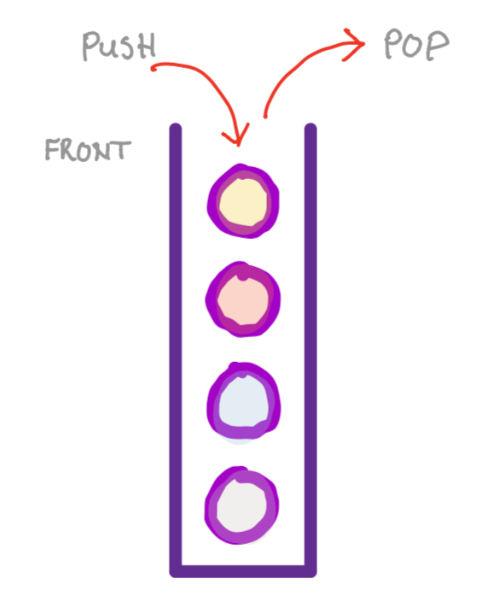
\includegraphics[width=\linewidth]{figures/stack-animation}
		\caption{Stack visualized}
	\end{minipage}
\end{figure}

\subsubsection{Push/Pop Visualization}
\begin{figure}[H]
		\centering
		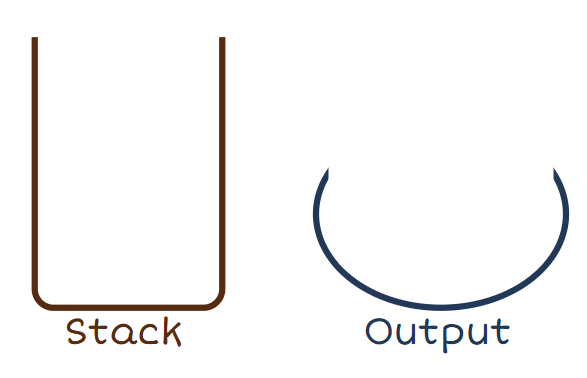
\includegraphics[width=0.45\textwidth]{figures/empty-stack}
		\caption{Create an Empty stack}
\end{figure}
\begin{figure}[H]
	\centering
	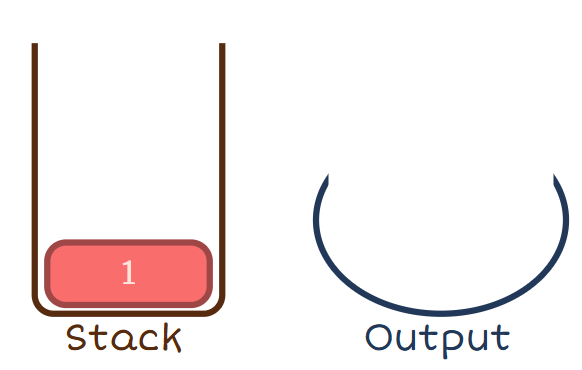
\includegraphics[width=0.45\textwidth]{figures/push-1}
	\caption{Push in the first element}
\end{figure}
\begin{figure}[H]
	\centering
	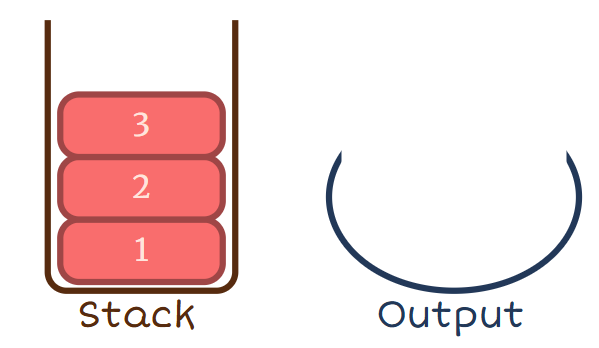
\includegraphics[width=0.45\textwidth]{figures/push-2-3}
	\caption{Push in the second and third element}
\end{figure}
\begin{figure}[H]
	\centering
	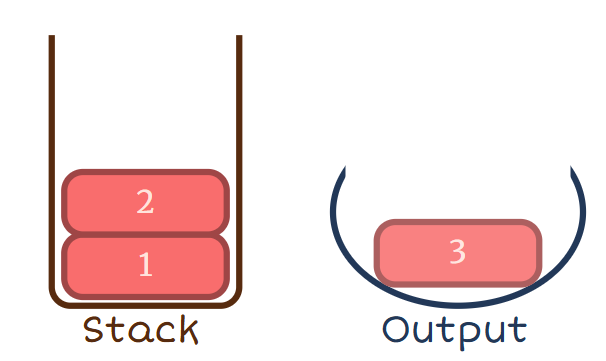
\includegraphics[width=0.45\textwidth]{figures/pop-3}
	\caption{Pop out the element at the top of the stack}
\end{figure}

\subsubsection{Coding}
\begin{lstlisting}[language=python, caption={Define Stack data structure class}]
	class MyStack:
		def _init_(self, capacity):
			self._capacity = capacity
			self._stack = []
			
		def push(self, value):
			if self.is_full():
				print('Do nothing!')
			else: 
				self._stack.append(value)
				
		def pop(self):
			if self.is_empty():
				print('Do nothing')
				return None
			else:
				return self._stack.pop()
			
		def print(self):
			print(self._stack)
			
		def is_full(self):
			return len(self._stack) == self._capacity
\end{lstlisting}

\begin{lstlisting}[language = python, caption={Push and Pop example}]
	stack1 = MyStack(5)
	stack1.push(12)
	stack1.push(8)
	stack1.push(21)
	stack1.push(33)
	stack1.push(34)
	stack1.push(35)
	stack1.print()
	
	//Output: Do nothing!
			  [12, 8, 21, 33, 34]	  
\end{lstlisting}

\subsection{Queue}
\subsubsection{Queue Visualization}
\begin{figure}[h]
	\centering 
	\begin{minipage}[b]{0.45\textwidth}
		\raggedright
		Queues return elements in the order in which they were stored. We call this kind of data structure first-in-first-out (FIFO).
	\end{minipage}
	\hfill
	\begin{minipage}[c]{0.3\textwidth}
		\centering
		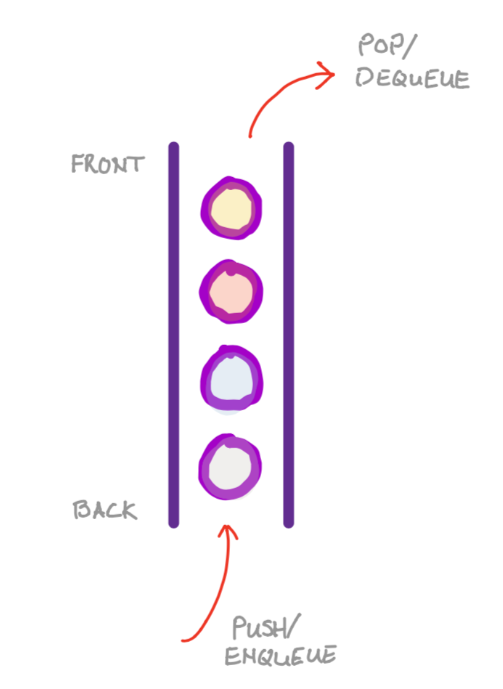
\includegraphics[width=\textwidth]{figures/queue-animation}
		\caption{Queue visualized}
	\end{minipage}
\end{figure}

\subsubsection{Queue/Dequeue Visualization}
\begin{figure}[H]
	\centering
	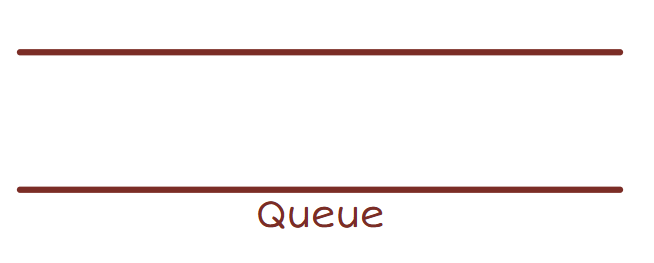
\includegraphics[width=0.45\textwidth]{figures/empty-queue}
	\caption{Create an Empty Queue}
\end{figure}
\begin{figure}[H]
	\centering
	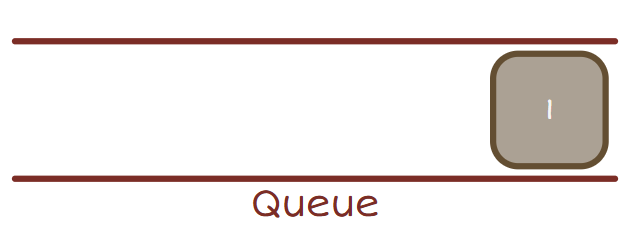
\includegraphics[width=0.45\textwidth]{figures/queue-1}
	\caption{Enqueue the first element}
\end{figure}
\begin{figure}[H]
	\centering
	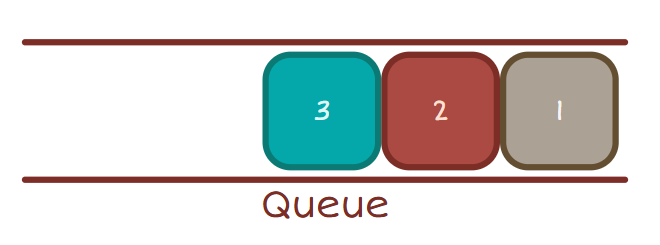
\includegraphics[width=0.45\textwidth]{figures/queue-2-3}
	\caption{Enqueue the second and third element}
\end{figure}
\begin{figure}[H]
	\centering
	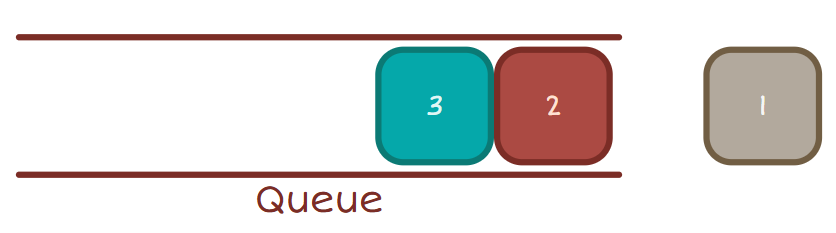
\includegraphics[width=0.45\textwidth]{figures/dequeue}
	\caption{Dequeue the element at the front of the queue}
\end{figure}

\subsubsection{Coding}
\begin{lstlisting}[language = python, caption={Define Queue data structure class}]
	class MyQueue:
		def _init_(self, capacity):
			self._capacity = capacity
			self._data = []
		
		def is_empty(self):
			return len(self._data) == 0
			
		def dequeue(self):
			if self.is_empty():
				print('Do nothing')
				return None	
			else: 
				return self._data.pop(0)
		
		def print(self):
			print(self._data)
\end{lstlisting}

\begin{lstlisting}[language = python, caption={Example}]
	queue = MyQueue(5)
	queue.print()
	
	queue.enqueue(9)
	queue.enqueue(5)
	queue.enqueue(2)
	queue.enqueue(1)
	queue.enqueue(0)
	queue.enqueue(6)
	
	//Output:
	Do nothing!
	[9, 5, 2, 1, 0]
\end{lstlisting}

	
	\chapter{Unix and Docker}
	
\end{document}
